\chapter{Literature}
    In this chapter, some basic knowledge of deep learning neural network for vision tasks, i.e. keypoints detection, will be introduced at the beginning. 
    More specifically, Some works about Wire harness detection using AI method will be presented. Additionally, some state of the art methods and architectures, 
    which might improve the precision of keypoints detection of wire harnessed will also be presented. After that, some approaches for generating datasets 
    artificially and expanding datasets are introduced at the end.
\section{Deep neural network for vision tasks}
    Recently, using deep neural network for vision tasks becomes a popular choice for researchers, for example, Image Classification\cite{8016501}, 
    Object detection\cite{10028728}, Human pose estimation\cite{Sun_2019_CVPR}, Semantic Segmentation\cite{HAO2020302}. Compare with the some 
    tradition computer vision technologies, the approach provide more satisfactory results\cite{voulodimos2018deep}. 
    In this section, some of the most important deep learning network structures for vision tasks will be introduced. Object and keypoints
    detection will be the highlights due to their close connection with the tasks of the thesis.\\
\subsection{Object detection and segmentation}
    The goals of object detection are: what(classification) and where(locolization) is the object is. \autoref{fig:object detection} is an example of object
    detection. In this image, the branches of wire harness is bounded by a green box as groundtruth. They are classified as branches and the locations could 
    also be detected. It serves as the basic of some deep learning based computer vision task such as instance segmentation and object tracking\cite{10028728}. 
    \begin{figure}
        \centering
        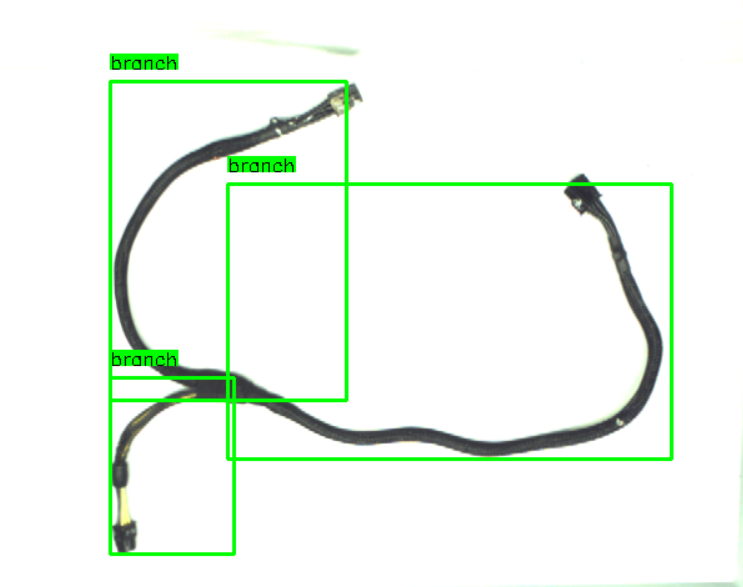
\includegraphics[width=0.6\linewidth]{example_images/object detection}
        \caption{Ground truth of Object detection}
        \label{fig:object detection}
    \end{figure}
    In \cite{Girshick_2014_CVPR}, the authors present a method called R-CNN(Region-based Convolutional Network), which improves the accuracy of object detection. 
    The approach consists of three modules:
    \begin{itemize}
        \item [(1)] \textbf{Region proposals: }In this module, category-independent region proposals will be generated.
        \item [(2)] \textbf{Feature extractions: }The features will be extracted using CNN \cite{NIPS2012_c399862d}.
        \item [(3)] \textbf{Classification: }At last the classification task is done by a set of classspecific linear SVMs. 
    \end{itemize}
    After one years, Ross Girshick proposed an optimized method named Fast R-CNN in 2015\cite{Girshick_2015_ICCV}. Compared with all objects on image are passed 
    through the neural network in R-CNN,  in Fast R-CNN the whole images will be passed forward together to extract the features, which improves the efficiency 
    significantly. Faster R-CNN combined Fast R-CNN with Region Proposal Networks(RPN), which outputs a set of rectangular object proposals, each with an objectness
    score\cite{NIPS2015_14bfa6bb}. It is trained end-to-end to generate high-quality region proposals, which are passed to Fast R-CNN for object detection tasks.
    This method simplified the process further and the model is easier to be trained.\\
    The above introduced models are from R-CNN family. Joseph Redmon proposed a new model named YOLO, whose pipeline has just one simple network. It could also be 
    trained end-to-end extremely fast\cite{Redmon_2016_CVPR}. The detection task will be framed as a regression problem to spatially separated bounding boxes and
    associated class probabilities. Due to the rapidity, it is widely used in the task of real-time object detection. After an eight-year development, the Tsinghua 
    University team presented the tenth generation of the YOLO model in 2024\cite{wang2024yolov10}. Today, the YOLO model integrates state-of-the-art deep learning 
    techniques, such as an enhanced version of CSPNet\cite{Wang2019CSPNetAN} as the backbone network, PAN (Path Aggregation Network) for effective multi-scale feature
    fusion\cite{Liu_2018_CVPR}. This enables fast and accurate real-time object detection.
    Kaiming He from Facebook AI Research extended Faster R-CNN\cite{NIPS2015_14bfa6bb} with a new branch for predicting the mask of objects\cite{He_2017_ICCV}. Therefore, it is widely 
    used in the field of instance segmentation. This method has also two stages. The predictions of mask and classification are in parallel. This is different from 
    the traditional method, as the previous method employed the predicted mask for classification. 
    \cite{10260646} is an implementation of mask RCNN for instance segmentation of the wire harness. It predicts the topology features such as overlapping points and branch
    points. These extracted features are then used for topology matching with their sensor representations.\\
\subsection{keypoints detection}
    While the object detection are powerful to classify and localize the instances keypoints detection has several advantages: (1) it has less computational effort, which
    is better for real-time detection. (2) It is more useful for some specific task, for example grabbing the wire harness, as the actuator needs the precise position of the grabbing point
    on wire harness. (3) It is easier for collecting the datasets, only several keypoints are needed to be annotated. This is quite helpful because there are almost no open 
    source harness datasets available.\\
    There are two main approaches for keypoints detection: Keypoint regression strategies and Heatmap regression strategies. 
    \begin{itemize}
        \item [(1)] \textbf{Keypoint regression strategies: } This is the direct method for keypoints detection. The position of key points, such as joints, is directly 
        regressed by coordinates\cite{Toshev_2014_CVPR}. In \cite{9710108}, Li and Bian point out the shortcomings of this approach: it suffers from inferior performance. 
        In challenging cases like occlusions, motion blur, and truncations, the ground-truth labels are inherently ambiguous. They proposed an optimized approach named  
        Residual Log-likelihood Estimation(RLE), which leverages normalizing flows to estimate the underlying distribution and boosts human pose regression. The novel 
        proposed method is more easily trainable than the traditional method.

        \item [(2)] \textbf{Heatmap regression strategies: } This is indirect method for keypoints detection. The likelihood heatmap of each joint will be generated and positions 
        are regressed by the maximum likelihood\cite{10.1007/978-3-319-46484-8_29}. Two drawbacks of this method are list in\cite{Sun_2018_ECCV}: 1) The likelihood-maximum equation, 
        see \autoref{eq:maximum likelihood}, is non-differentiable. 2) the heat map representation leads to quantization error.
        \begin{align}
            J_{k}=arg\max_{p}H_{k} (p)
             \label{eq:maximum likelihood}
        \end{align}
        The first problem about the non-differentiable equation could lead to non-end-to-end training. The author presented an optimized method called integral pose regression, which
        allows end-to-end training, has continuous solutions and no quantization problem. They normalized the heatmaps by softmax to get $\widetilde{H}_{k}$ at the beginning and weighted 
        them by their probabilities p \autoref{eq:soft maximum likelihood}, where $\Omega$ is the domain.\\
        \begin{align}
            J_{k}=\int_{p\in \Omega } p\cdot \widetilde{H}_{k}(p) 
             \label{eq:soft maximum likelihood}
        \end{align}
    \end{itemize}
\subsection{Backbones and necks for vision tasks}
    The state-of-the-art deep learning models for vision tasks usually consist of three modules: backbone, neck and head\cite{Bouraya2021}. It starts from the input image and hierarchical 
    features are then extracted by the backbone. The Neck will aggregate multi-scales features and prepare for the task-specific prediction, which is then performed in the head, e.g., 
    classification and segmentation. In this subsection, some state-of-the-art backbones and necks for vision tasks will be introduced.
\subsubsection{Backbones}
    In \cite{simonyan2015a}, the team from University of Oxford uses very simple structure to extract the deep features of the input image. The image passes through a stack of convolutional 
    layers, which has 3x3 kernels. The max-pooling layer follows some convolutional layers. This structure is very simple and widely used as baseline in some later works\cite{guan2019deep}
    \cite{tammina2019transfer}. The ResNet family is popularly used for extracting features in vision tasks. Resnet-50\cite{7485869} is one of the most popular backbones for computer vision 
    tasks. The depth of representations is of central importance for many visual recognition tasks. A so-called residual learning framework is presented to improve the depth of the network.
    With the depth of neural network increasing, some challenges, like degradation and gradient vanishing, have also been exposed. Instead of learning the desired mapping $H(x)$ directly, 
    The residual block learns another mapping $H(x) - x$, which is easier to be optimized. Resnet made it possible to train extremely deep networks, which led to significant progress in 
    computer vision.\\
    \textbf{Transformer in backbones: }\cite{7803544} uses encoders to capture the features of interest with convolutional layers. The core of its structure is the hierarchical decoders 
    which upsample the low-resolution input feature maps with max-pooling to reconstruct. This structure has a good trade-off between accuracy and memory but due to the compression of input, 
    a lot of information is lost and the longer the input sequence, the worse the problem becomes. To solve this problem, Vaswani proposed a new architecture, Transformer which is also based 
    on encoder-decoder architecture but integrals attention mechanism allowing modeling of dependencies without regard to their distance in the input or output sequences \cite{NIPS2017_3f5ee243}.
    In contrast to traditional encoder-decoder architecture, the transformer uses Multi-Head Attention followed by a simple, position wise fully connected feed-forward network as an encoder 
    to compute representations from input sequences and the decoder inserts an additional Multi-head attention to connect the output of encoders. 
    The transformer is initially applied for textual information and currently, some researchers have also adapted it to deal with vision tasks as well.
    \cite{dosovitskiy2021an} proposed a method called Vision Transformer(ViT), which directly implied transformer for vision tasks. The traditional transformer processes sequences of words,
    while ViT divides the image into patches and uses the attention mechanism to find dependencies between different patches. The patches of the image could then be interpreted as the words 
    in the traditional method. The images are divided into different with the fixed size (16x16), which means that it has a high computational complexity. Because each individual patch has 
    to compute attention with the every other patch. This is one of the drawbacks of ViT. In \cite{9710580}, Swin-Transformer is presented. Instead of the fixed patch size,  Swin-Transformer
    divided the image into some "local windows", e.g., a 7x7 patches. It reduces significantly the computational complexity. To gain the intetactions between different local windows, 
    Swin-Transformer shifted the windows in different layers. Compare with single size feature maps of ViT, Swin-Transfomer starts from the small patches and merges them in deeper layers. Hence,
    Swin-Transformer also has hierarchical features, which is similar with the convolutional based backbones like Resnet. This is good for aggregating multi-scales features in the following part.
\subsubsection{Necks}
    Feature Pyramid Networks (FPN)\cite{8099589} and U-Nets\cite{10.1007/978-3-319-24574-4_28} are two successful neural networks to integrate the feature maps of different scales.
    FPN contain two pathways: bottom-up and top-down respectively. The feature parameters 
    of the input image are extracted by the backbones and output proportionally sized feature maps at multiple levels with a scaling step of two in the bottom-up pathway. 
    In the top-down pathway, the low-level feature map is added with the high-level feature map element-wise after upsampling. This process enhances the semantic strength 
    of the features for better prediction. This process is independent of the backbone convolutional architectures, and in this paper, the author uses ResNet to extract features.
    U-Net has an encoder-decoder structure. The encoder contracts the size of the image 
    and increases the feature channels through max pooling, while the decoder performs the opposite pathway through up convolution. Concatenation with the correspondingly 
    cropped feature map from the contracting path is necessary to prevent the loss of border pixels in up convolution. The differences between U-Net and FPN are as follows:
    \begin{itemize}
    \item [1)] FPN integrates feature maps of different scales through element-wise addition, while U-Net integrates through concatenation.      
    \item [2)] FPN predicts through every feature map in the top-down pathway, while U-Net only does prediction at the final layer.
    \item [3)] FPN enlarges the feature map through nearest neighbor upsampling in the top-down pathway, while U-Net uses up convolution. 
    \item [4)] FPN's low-level features are the same size as the high-level features when upsampled by a factor of 2, whereas in U-Net 
    they are usually not, requiring cropping on the low-level features to match the scaled-up high-level features.
    \end{itemize}
\section{Wire harness detection} 
    In order for an actuator to be able to operate the wire harness instead of the human, it needs to be accurately localized. In contrast to rigid objects, the BDLOs' degree 
    of freedom is infinite. So their geometrical configuration changes during manipulation, which poses great challenge for automatic manipulation\cite{9665147}. 
    The wire harness consists of k branches. The first node has no parents, whereas all 
    following nodes have exactly one parent node\cite{10161483}. To localize the harness and reconstruct the topology, every individual branch should be localized precisely. 
    However, after localization, some parts of the branch are still missing. Several researchers have proposed approaches to improve the accuracy of localization and topology reconstruction. 
    There are mainly two approaches: 
    \begin{itemize}
        \item [1)] Use initially good estimated model of wire harness to track the obtained point cloud from the camera.
        \item [2)] Use deep learning segmentation method to obtain a mask of the wire harness.
    \end{itemize}
\subsection{Registration through pre-knowledge of wire harness} \label{Registration through pre-knowledge of wire harness}
    Two stereo cameras are used to localize the wire harness 
    on workbench in \cite{10.1007/978-3-031-27933-1_31}. The first camera obtained the rough localization of the wire harness. The second camera will move over the rough estimated position 
    obtained from the first camera and the individual component of interests on wire harness could be localized, which allows a high resolution pose estimation. This approach could estimate 
    the position of target component precisely if there is a sufficiently good estimate of the initial configuration to perform successful registration.
    In \cite{doi:10.1177/0278364919841431}, the researcher presents a method for the registration called Structure Preserved Registration (SPR), where each object node is regarded as a Gaussian 
    centroid, and the point cloud is one dataset sampled from the mixture Gaussians. Through the maximum likelihood estimation for the registration with the sampled point cloud to obtain the 
    best estimation of the node positions, i.e., the centroids of the Gaussian. In expectation step(E-step), it computes the posterior probability that the point cloud is assigned to the
    centroid through by using the centroid position and variance from the previous step. In maximization step(M-step), the likelihood is maximized to obtain the best estimation of the centroid position 
    and variance. These two steps are iterated until the log-likelihood function is converged. The presented method could track deformable objects without branch accurately, robustly, and efficiently. 
    In \cite{9665147}, a modification to the method of SPR is proposed to enhance its capability for tracking DLOs with multiple branches. This modified method releases the SPR's problem of incorrect 
    registration of branches by introducing branch-wise probability estimates in the underlying Gaussian Mixture Model. In \cite{10161483}, Manuel proposed a method for matching the topology of a branched 
    deformable linear object to camera sensor data. Features are extracted from camera images to construct a graph-based topology representation, which is matched to a graph-based topology 
    representation of the known branched deformable linear object. The matching cost function is defined as the difference between the modeled topology 
    and the estimated topology and is minimized to obtain optimal mapping, but it is only implemented for non-overlapping wire scenarios.
\subsection{Wire harness segmentation}
    The registration method could track the point clouds to localize the wire harness precisely and robustly. However, it has also two drawbacks: (1) It needs previous knowledge of the 
    wire harness. (2) It suffers from the problem of overlapped branches, which is common for wire harness. Many scientists have focused on developing segmentation method to avoid these 
    problems. \cite{Caporali2022}, an algorithm called FASTDLO is presented. The image of deformable linear objects(DLOs) is processed initially with a deep convolutional neural network for background segmentation 
    to obtain a binary mask. After obtaining endpoints, sections, and intersections through skeleton pixel classification, which are keypoints of the DLOs, segments are generated, 
    but intersection-relative areas are discarded. With a shallow neural network, connection probabilities are predicted, and the discarded areas are processed. Segments are then 
    concatenated, intersections are reconstructed, and covered with RGB colors. In this paper, the problem of overlapping is overcome.
\subsection{Spline representation}
    The segmentation method has high complexity of computation, which is not suitable for real-time detection. Instead of segmenting the whole pixel of DLOs, in \cite{degregorio2018lets}
    the author just analyzes some super pixels, i.e., super pixels. The best path between the seed points will be found through some similar features of DLOs, e.g, similarity of appearance as well as 
    curvature. It allows to compute the most compatible b-spline of each object.
    In \cite{10167643}, the author points out that FASTDLO
    was struggled to solve some really complicated scenes of DLOs, e.g., high curvature and many overlaps and intersections. In addition, although the super-pixel method has a 
    high accuracy, but it has a big number of hyperparameters and requires the DLOs with the same color. Another robust algorithm 
    for real-time detection of DLOs is presented, capable of producing an ordered pixel sequence of each DLO’s centerline along with segmentation masks. In contrast to FASTDLO, it 
    handles intersections robustly by choosing the combination of paths that minimizes the cumulative bending energy of the DLO(s). The branch points are important for the skeleton 
    but could improve the complexity of the problem for the walker to choose the possible path. To avoid this, in \cite{10160437}, the author removes 
    the branch points after the skeleton and postpones the decision for further processing. So initially only the endpoints are considered, and the walker starts from one 
    of them till arriving at the other one. After walking through all segments and ordering, a sequence of knot points is extracted to determine the b-spline. Compared to the previous 
    FASTDLO and super-pixel methods, it does not need deep learning model and decrease the computational complexity further. 
\section{Dataset expansion}
    In contrast to unsupervised learning, supervised learning requires a large dataset to train the model. It plays the role of teaching the model to learn the desired knowledge.
    If the dataset for training is too small, then there is a risk of overfitting, i.e., the dataset is too small or too simple for the model, which is not good for generalization.
    However, the experts suffer from annotating the original data, because it is time-consuming and inefficient. Scientists have explored different paths to expand the dataset 
    for a better training. 
\subsection{Synthesized dataset}
    Collecting real data is difficult, but combining with the known features of the target and Synthesizing the dataset artificially are simpler. The background of the object in the 
    image will strongly influence the detection. 
    In \cite{9349395}, Riccardo proposes an approach that uses an image of the target object placed in front of a monochromatic background. By employing the chroma-key technique,
    it can easily obtain the masks of the target object and replace the background to produce a domain-independent dataset. In \cite{Tremblay_2018_CVPR_Workshops}, Jonathan combines 
    both to synthesize datasets, which were generated by placing 3D household object models in virtual environments. Besides changing the environment of an object, the objects are 
    also changed through translation and rotation. In \cite{8972568}, the authors train the neural network with the rendered spline curve to detect the real spline. Although this 
    method is easy to be implemented, but there is still a gap between the rendered and the real spline. e.g., lighting, texture on the spline. They have developed a method to minimize
    the gap without groundtruth. The state of the spline is estimated by a differentiable render as membership weights. The membership weights present the possibilities, weather each 
    pixel belongs to the spline or the background. Implement the M-step of GMM method, which is mentioned in \ref{Registration through pre-knowledge of wire harness}, to estimate the 
    GMM parameters such as the centroid position and variance. In E-step, the new membership weights will be calculated to replace the old weight. Because the computerized tomography(CT) 
    images have higher accuracy and are easier to be segmented, so in \cite{SONG2022106706}, Song wants using transfer learning to optimize the segmentation of ultrasound(US) images. But 
    there are also a big gap between these two kind of images, thus transfer learning is difficult to be implemented. The cycle generative adversarial network (CycleGAN) is used to map the 
    CT images to US images and doesn't need annotated dataset. The synthesized US images have the features of the real images. After the training with the synthesized images, the model is 
    trained and fine-tuned with the real US images. The result shows that it improves the accuracy of segmentation of US images significantly. 

